\chapter{Λογιστική Παλινδρόμηση}
\label{appendix:LReg}
Σκοπός αυτού του αλγορίθμου δεν είναι ακριβώς να ταξινομήσει τα δεδομένα, αλλά να δώσει πιθανότητες σε κάθε κλάση δεδομένων των χαρακτηριστικών.
\paragraph{Η λογιστική συνάρτηση.} Η συνάρτηση αυτή παίρνει τιμές από $- \infty$ μέχρι $+ \infty$ και δίνει έξοδο μεταξύ $0$ και $1$, άρα μπορούμε να την ερμηνεύσουμε ως πιθανότητα. Δίνεται από τον τύπο:
$$\theta(s)=\frac{e^s}{1 + e^s}$$
\begin{figure}[H]
	\centering			
%	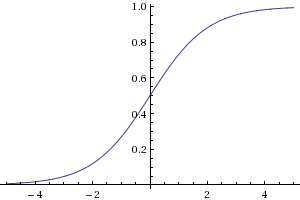
\includegraphics[width=0.6\textwidth]{logistic.png}
	\caption[Η λογιστική συνάρτηση]{Η λογιστική συνάρτηση}
\end{figure}

\paragraph{Ερμηνεία} Καθώς θέλουμε να κάνουμε μια πρόβλεψη για κάποιο άγνωστο χαρακτηριστικό με βάση κάποια άλλα χαρακτηριστικά-προβλέπτες που το αφορούν κινούμαστε στα εξής πλαίσια: αρχικά υπολογίζουμε πως επηρεάζει κάθε χαρακτηριστικό-προβλέπτης την άγνωστη ποσότητα, δηλαδή του δίνουμε κάποιο βάρος. Στη συνέχεια με βάση τα χαρακτηριστικά ενός δεδομένου παίρνουμε μία τιμή
για αυτό, την οποία θα μπορούσαμε να ερμηνεύσουμε ως το βαθμό που εμφανίζει το δεδομένο ως προς το χαρακτηριστικό που προβλέψουμε. Στη συνέχεια περνάμε αυτή τη τιμή  από ένα κατώφλι, ώστε να δούμε πού θα την κατατάξουμε. Η μαθηματική μετάφραση της παραπάνω διαδικασίας είναι η εξής:
$$s=w^T x \rightarrow h(x)=\theta(s)=\frac{e^{w^T x}}{1 + e^{w^T x} }$$
Η πραγματική πιθανότητα, που προσπαθούμε να προσεγγίσουμε  ορίζεται ως εξής:
$$P(y \mid x)=\left\{
\begin{array}{ll}
f(x)  & \mbox{if } y = +1 \\
1 - f(x)  & \mbox{if } y = -1
\end{array}
\right.$$

Αν υποθέσουμε πως η υπόθεσή μας είναι σωστή, δηλαδή $h=f$, τότε η πιθανότητα να πάρουμε έξοδο y για ένα δεδομένο με χαρακτηριστικά x είναι:
$$P(y \mid x)=\left\{
\begin{array}{ll}
h(x)  & \mbox{if } y = +1 \\
1 - h(x)  & \mbox{if } y = -1
\end{array}
\right.$$

Αν αντικαταστήσουμε με $h(x)=\theta(w^T x)$ και λαμβάνοντας υπόψιν πως $\theta(-s)= 1 - \theta(s)$, τότε η πιθανότητα  προκύπτει:
$$P(y \mid x)= \theta(y w^T x)$$
Ο παραπάνω τύπος λαμβάνει υπόψιν του μόνο ένα σημείο. Αν έχω N δεδομένα στο σετ εκπαίδευσης τότε η υπόθεσή μου γίνεται:
$$\prod_{n=1}^{N} P(y \mid x)= \prod_{n=1}^{N} \theta (y_n w^t x_n)$$
Η ερώτηση την οποία οφείλουμε να απαντήσουμε τώρα είναι : ”Δεδομένου του σετ εκπαίδευσης, ποιά είναι η πιθανότερη υπόθεση;” Η συνάρτηση, την οποία θέλουμε να ελαχιστοποιήσουμε, είναι η εξής:

$$Error(w)= \frac{1}{N} \sum_{n=1}^{N} \ln (1 + e^{- y_n w^T x_n} )$$

\paragraph{Gradient descent} Πρόκειται για έναν αλγόριθμο βελτιστοποίησης που προσπαθεί να βρει το τοπικό ελάχιστο μιας κυρτής συνάρτησης. Η διαδικασία είναι επαναληπτική και σε κάθε βήμα ο αλγόριθμος επιλέγει άπληστα να κινηθεί προς την πιο απότομη κατεύθυνση, που αντιστοιχεί στην αντίθετη κατεύθυνση της κλίσης στο συγκεκριμένο σημείο.
\begin{figure}[H]
	\centering			
%	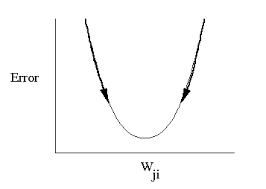
\includegraphics[width=0.6\textwidth, height=5cm]{gradient.png}
	\caption[Steepest descent]{Steepest descent}
\end{figure}
Εκτός από την κατεύθυνση προς την οποία θα κινηθεί ο αλγόριθμος πρέπει να επιλέξει και το μέγεθος του βήματος που θα εκτελέσει. Η παράμετρος αυτή επηρεάζει τόσο την ταχύτητα εκτέλεσης του αλγορίθμου, όσο και την επιτυχία του: αν τα βήματα που κάνει είναι σταθερά και μικρά, τότε θα φτάσει εγγυημένα σε κάποιο ελάχιστο, αλλά πολύ αργά, μειώνοντας την απόδοση του συστήματος. Αντιθέτως αν το βήμα είναι πολύ μεγάλο, μπορεί να υπερπηδά το ελάχιστο κάθε φορά που το πλησιάζει και ο αλγόριθμος να μην συγκλίνει ποτέ. Συνήθως υιοθετούμε μια πιο σύνθετη προσέγγιση: επιλέγουμε αρχικά μεγάλο βήμα, ώστε να πλησιάσουμε γρήγορα στη λύση και το μειώνουμε μόλις φτάσουμε κοντά.
\begin{figure}[H]
	\centering
	\begin{minipage}{.5\textwidth}
		\centering
%		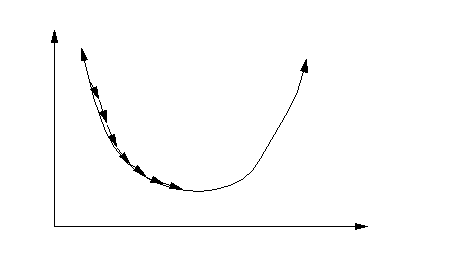
\includegraphics[width=0.8\linewidth, height=0.15\textheight]{smallstep.png}
		\caption[Gradient descent με πολύ μικρό βήμα]{Gradient descent με πολύ μικρό βήμα}
		
	\end{minipage}%
	\begin{minipage}{0.5\textwidth}
		\centering
%		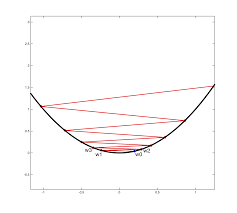
\includegraphics[width=0.8\linewidth, height=0.15\textheight]{bigstep.png}
		\caption[Gradient descent με πολύ μεγάλο βήμα]{Gradient descent με πολύ μεγάλο βήμα}
		
	\end{minipage}
\end{figure}